\chapter{Analyse}

\noindent Cette section présente une analyse détaillée de l'architecture et du fonctionnement de \textbf{SecuCom}. À travers différents diagrammes UML, nous allons explorer la structure du système, ses composants, les relations entre les entités, ainsi que les flux d'interactions entre les différents acteurs et le système.

\section{Diagramme de composants}

\noindent Le diagramme de composants ci-dessous illustre l'architecture modulaire de \textbf{SecuCom}, mettant en évidence les principaux modules du système, leurs sous-composants et leurs interactions.

\begin{figure}[H]
\centering
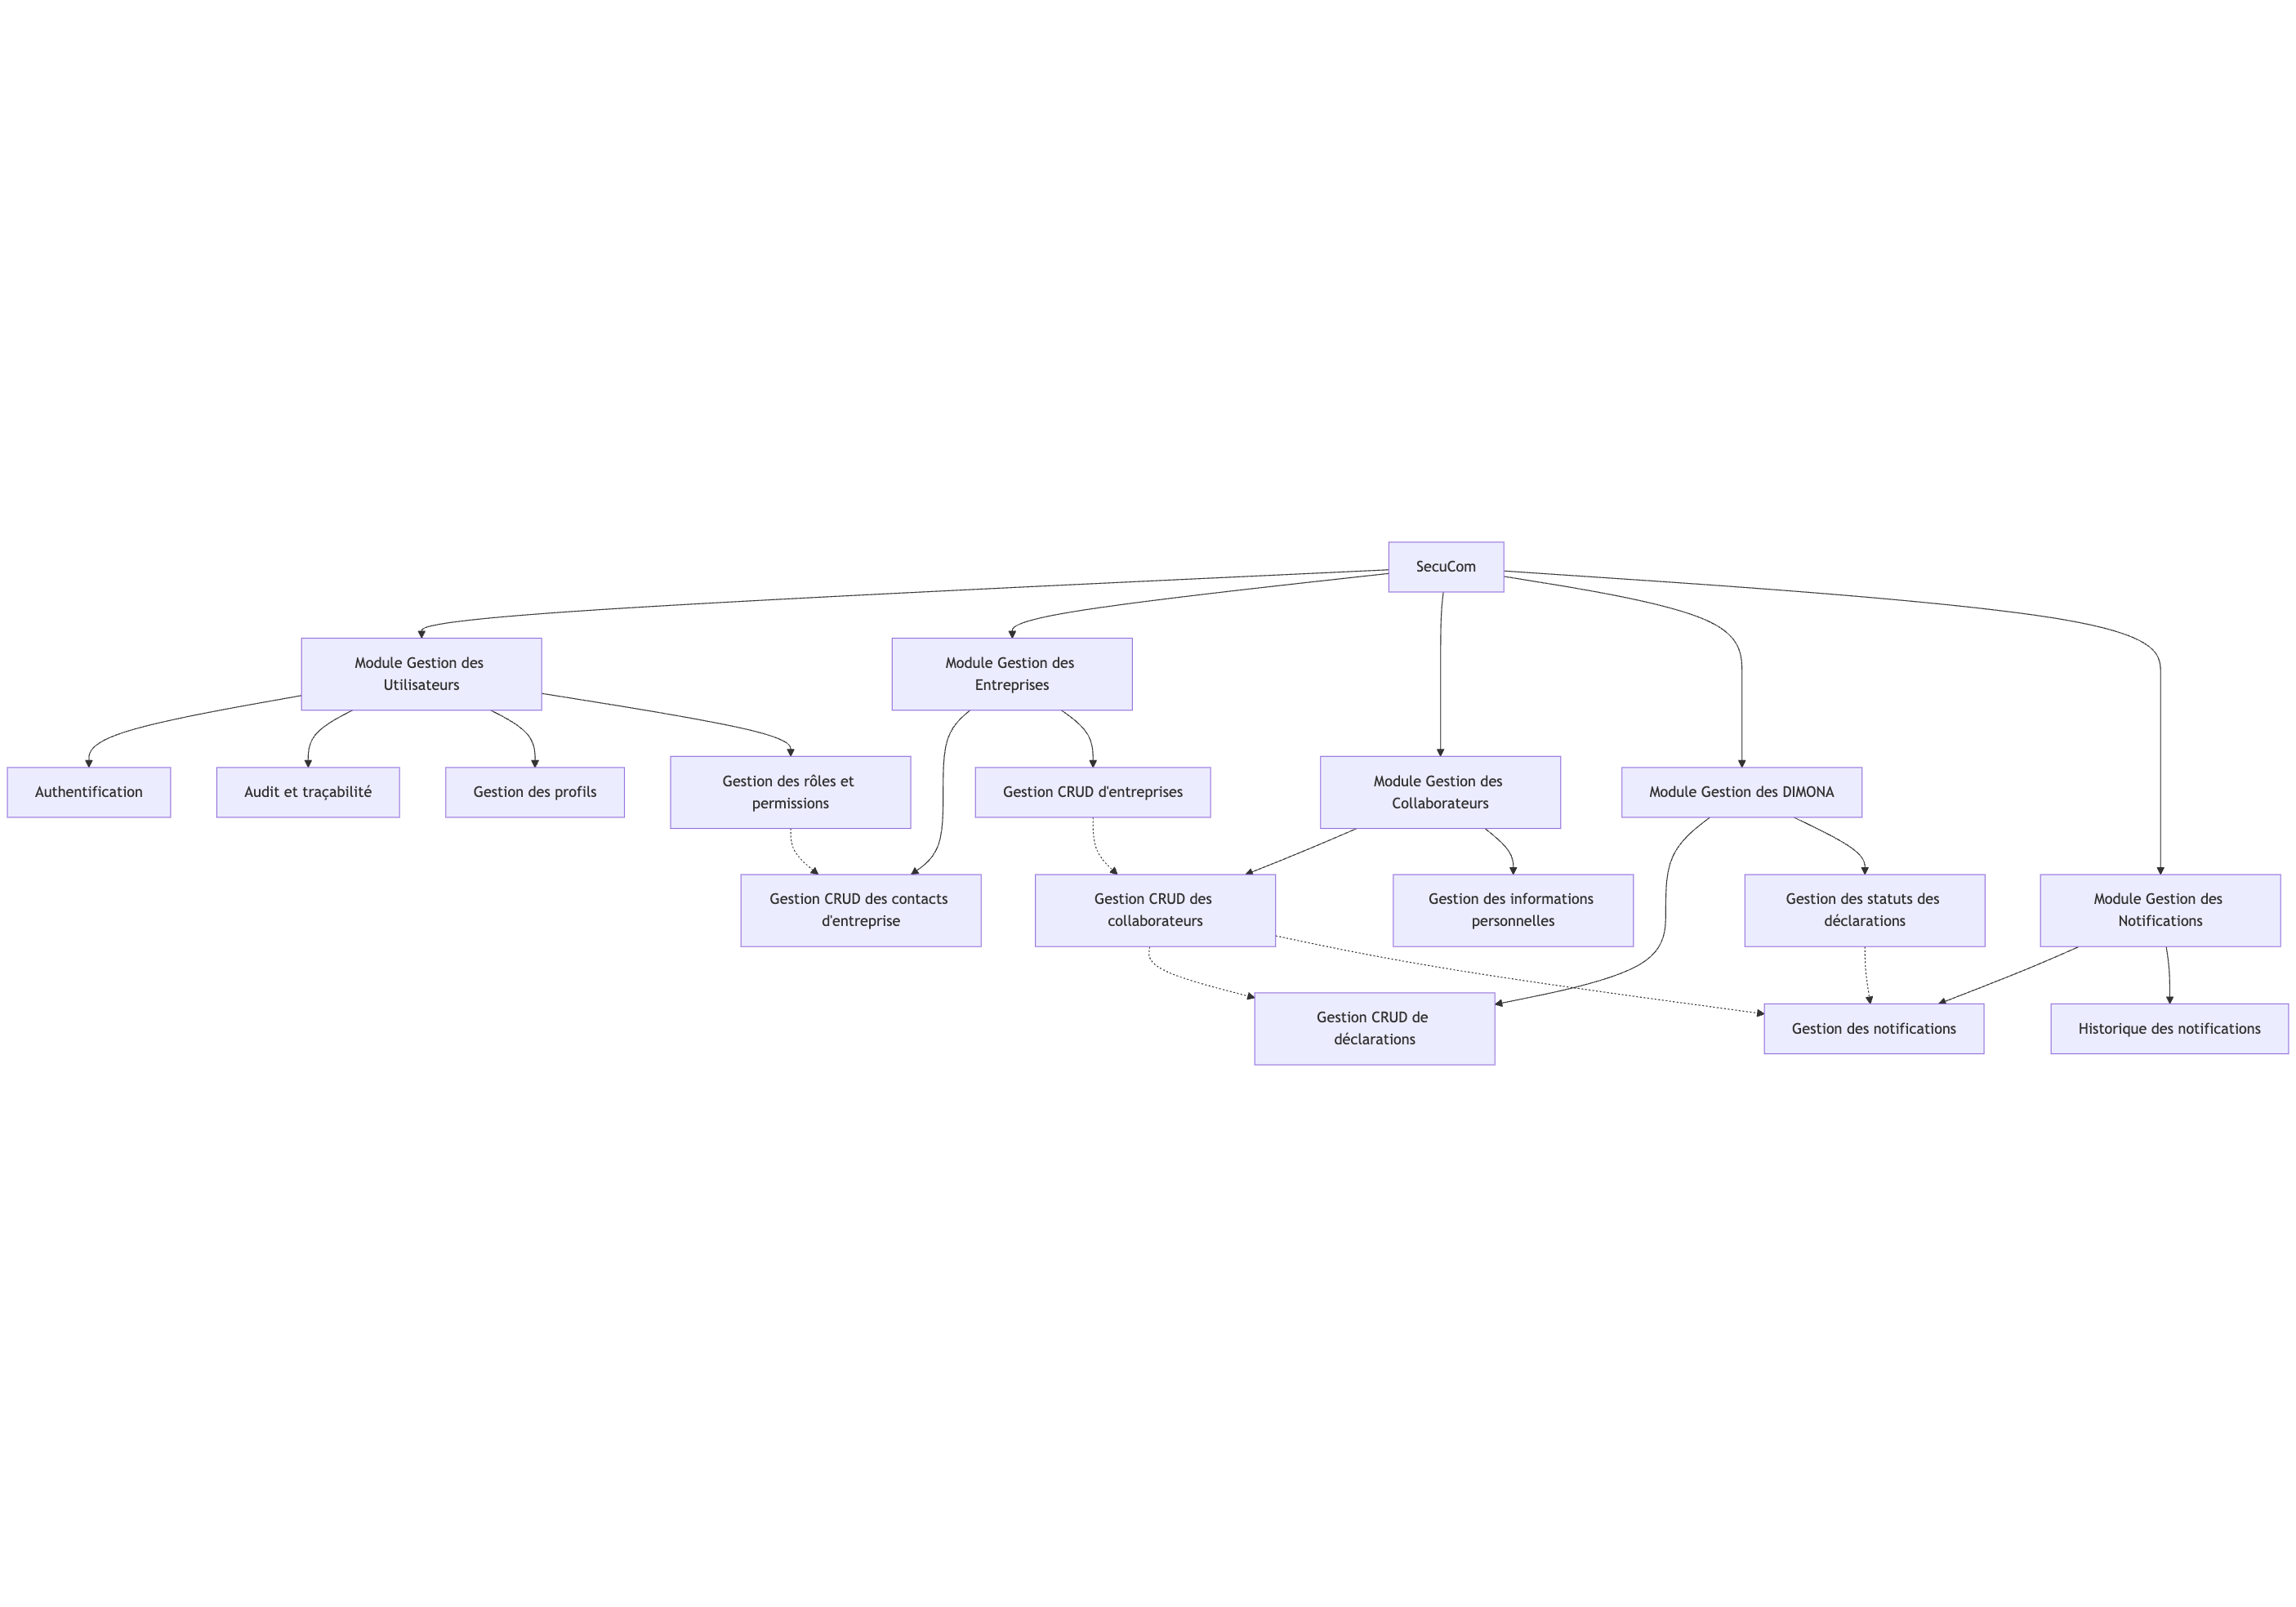
\includegraphics[width=0.9\textwidth]{ComposantsDiagram.png}
\caption{Diagramme de composants de SecuCom}
\end{figure}

\vspace{0.5cm}

\noindent Le système \textbf{SecuCom} est structuré autour de cinq modules principaux, chacun responsable d'un aspect spécifique de la plateforme :

\begin{itemize}[leftmargin=*,label=\textcolor{darkgray}{$\bullet$},itemsep=0.3em]
  \item \textbf{Module Gestion des Utilisateurs} : Comprend quatre sous-composants critiques :
    \begin{itemize}[leftmargin=*,label=\textcolor{darkgray}{$\bullet$},itemsep=0.3em]
      \item \textit{Authentification} : Gère la vérification des identités des utilisateurs.
      \item \textit{Audit et traçabilité} : Enregistre les actions des utilisateurs pour des fins de sécurité.
      \item \textit{Gestion des profils} : Permet la création, modification et suppression des profils utilisateurs.
      \item \textit{Gestion des rôles et permissions} : Définit et gère les droits d'accès aux différentes fonctionnalités.
    \end{itemize}
  
  \item \textbf{Module Gestion des Entreprises} : Comprend deux sous-composants essentiels :
    \begin{itemize}[leftmargin=*,label=\textcolor{darkgray}{$\bullet$},itemsep=0.3em]
      \item \textit{Gestion CRUD d'entreprises} : Gère le cycle de vie complet des entités entreprises (création, lecture, mise à jour, suppression).
      \item \textit{Gestion CRUD des contacts d'entreprise} : Administre les utilisateurs associés à chaque entreprise.
    \end{itemize}
  
  \item \textbf{Module Gestion des Collaborateurs} : Se compose de deux sous-composants :
    \begin{itemize}[leftmargin=*,label=\textcolor{darkgray}{$\bullet$},itemsep=0.3em]
      \item \textit{Gestion CRUD des collaborateurs} : Gère les travailleurs associés aux entreprises.
      \item \textit{Gestion des informations personnelles} : Administre les données personnelles des collaborateurs.
    \end{itemize}
  
  \item \textbf{Module Gestion des DIMONA} : Divisé en deux sous-composants :
    \begin{itemize}[leftmargin=*,label=\textcolor{darkgray}{$\bullet$},itemsep=0.3em]
      \item \textit{Gestion CRUD de déclarations} : Permet l'initiation, la consultation, la modification et la suppression des déclarations DIMONA.
      \item \textit{Gestion des statuts des déclarations} : Offre une visibilité sur l'état des déclarations en cours.
    \end{itemize}
    
  \item \textbf{Module Gestion des Notifications} : Comprend deux sous-composants :
    \begin{itemize}[leftmargin=*,label=\textcolor{darkgray}{$\bullet$},itemsep=0.3em]
      \item \textit{Gestion des notifications} : Gère l'envoi et le traitement des notifications.
      \item \textit{Historique des notifications} : Conserve un historique des notifications envoyées pour référence et suivi.
    \end{itemize}
\end{itemize}

\vspace{0.5cm}

\noindent Le diagramme met également en évidence des relations de dépendance importantes entre certains sous-composants :
\begin{itemize}[leftmargin=*,label=\textcolor{darkgray}{$\bullet$},itemsep=0.3em]
  \item La gestion d'entreprises (\textit{Gestion CRUD d'entreprises}) est liée à la gestion des collaborateurs (\textit{Gestion CRUD des collaborateurs}), illustrant le flux de travail où une entreprise doit exister avant de pouvoir y associer des collaborateurs.
  \item De même, la gestion des collaborateurs est liée à la gestion des déclarations DIMONA, reflétant la nécessité d'avoir un collaborateur enregistré avant de pouvoir effectuer une déclaration le concernant.
  \item La gestion des statuts des déclarations (\textit{Gestion des statuts des déclarations}) est liée à la gestion des notifications (\textit{Gestion des notifications}), permettant d'envoyer des notifications automatiques lorsqu'une déclaration DIMONA est créée ou change de statut.
  \item La gestion des collaborateurs (\textit{Gestion CRUD des collaborateurs}) est également liée à la gestion des notifications (\textit{Gestion des notifications}), permettant d'envoyer des notifications automatiques lorsqu'un nouveau collaborateur est créé.
\end{itemize}

\vspace{0.5cm}

\begin{tcolorbox}[
  title={\textbf{Architecture modulaire de SecuCom}},
  colback=blue!5!white,
  colframe=primarycolor,
  fonttitle=\bfseries,
  boxrule=0.5mm,
  arc=2mm,
  left=6mm,
  right=6mm,
  top=6mm,
  bottom=6mm
]
Cette architecture modulaire facilite la maintenance et l'évolution du système, chaque module pouvant être développé, testé et mis à jour de manière relativement indépendante, tout en préservant les interactions nécessaires entre les différentes fonctionnalités.
\end{tcolorbox}

\section{Diagramme de classes}

\noindent Le diagramme de classes ci-dessous représente les principales entités du système \textbf{SecuCom} et leurs relations. Il a été optimisé pour montrer clairement les classes actuellement utilisées dans l'implémentation et leurs relations.

\begin{figure}[H]
\centering
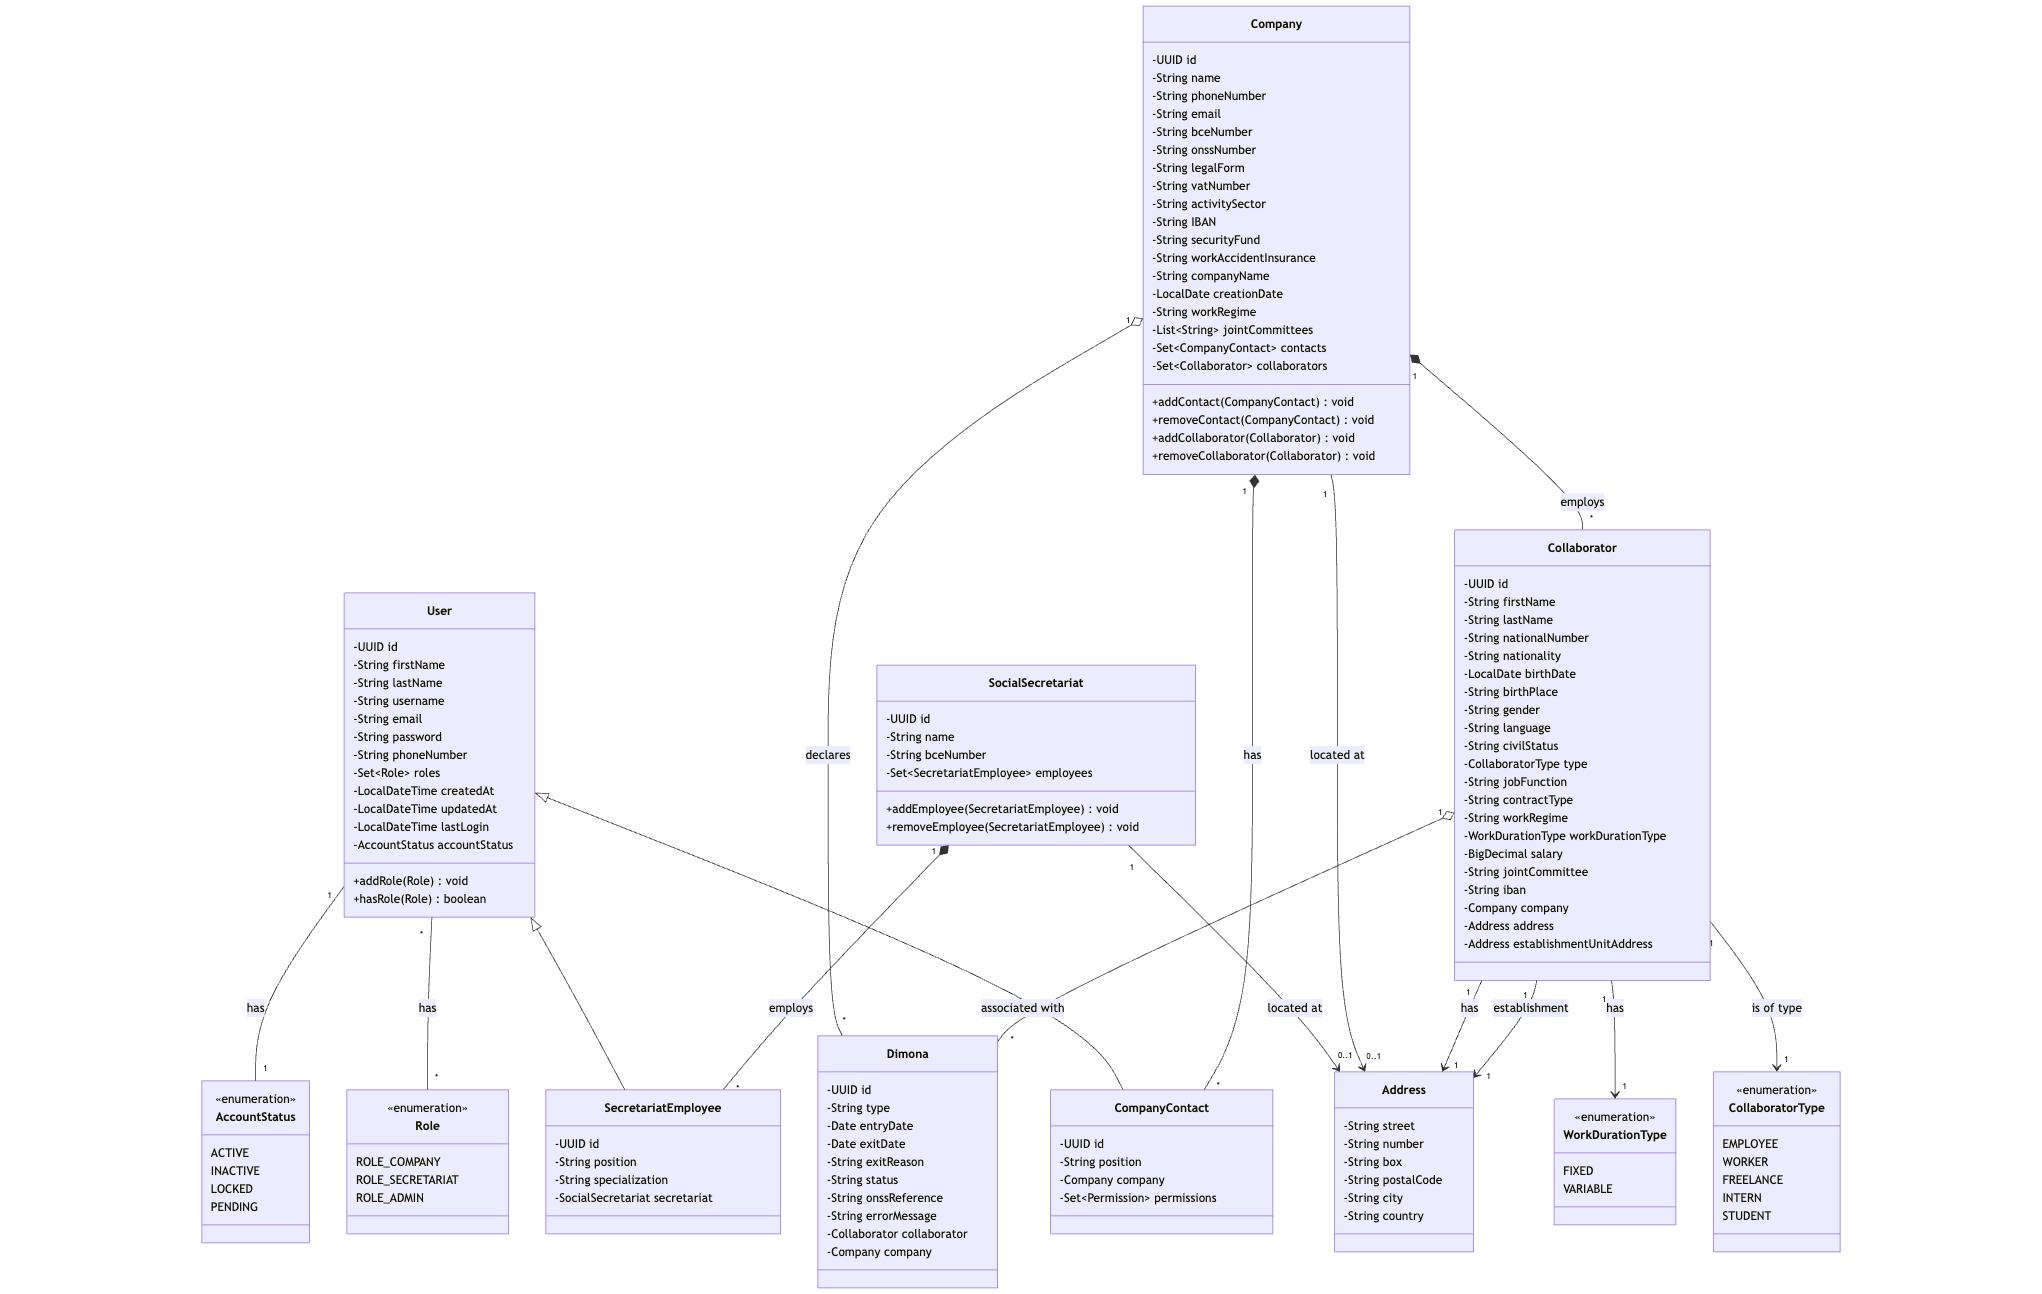
\includegraphics[width=0.9\textwidth]{ClassDiagram.png}
\caption{Diagramme de classes de SecuCom}
\end{figure}

\vspace{0.5cm}

\noindent Les principales classes du système sont :

\begin{itemize}[leftmargin=*,label=\textcolor{darkgray}{$\bullet$},itemsep=0.3em]
  \item \textbf{User} : Classe de base pour tous les utilisateurs du système, avec des attributs comme id, email, password, firstName, lastName, etc. Elle est associée à des rôles (Role) et à un statut de compte (AccountStatus).

  \item \textbf{Role} : Énumération définissant les différents rôles disponibles dans le système (ROLE\_COMPANY, ROLE\_SECRETARIAT, ROLE\_ADMIN).

  \item \textbf{AccountStatus} : Énumération définissant les différents états possibles d'un compte utilisateur (ACTIVE, INACTIVE, LOCKED, PENDING).

  \item \textbf{SocialSecretariat} : Représente le secrétariat social avec ses informations et ses employés. Il peut avoir plusieurs employés (SecretariatEmployee) et est associé à une adresse (Address).

  \item \textbf{SecretariatEmployee} : Employé du secrétariat social, hérite de User et est associé à un secrétariat social (SocialSecretariat).

  \item \textbf{Company} : Entreprise cliente avec ses informations d'identification et ses contacts. Elle peut avoir plusieurs contacts (CompanyContact), plusieurs collaborateurs (Collaborator) et plusieurs déclarations DIMONA (Dimona). Elle est également associée à une adresse (Address).

  \item \textbf{CompanyContact} : Contact au sein d'une entreprise cliente, hérite de User et est associé à une entreprise (Company).

  \item \textbf{Collaborator} : Travailleur d'une entreprise cliente avec ses informations personnelles et professionnelles. Il est associé à une entreprise (Company), à une adresse personnelle (Address), à une adresse d'établissement (Address), à un type de collaborateur (CollaboratorType) et à un type de durée de travail (WorkDurationType). Il peut avoir plusieurs déclarations DIMONA (Dimona).

  \item \textbf{CollaboratorType} : Énumération définissant les différents types de collaborateurs (EMPLOYEE, WORKER, FREELANCE, INTERN, STUDENT).

  \item \textbf{WorkDurationType} : Énumération définissant les différents types de durée de travail (FIXED, VARIABLE).

  \item \textbf{Dimona} : Déclaration DIMONA associée à un collaborateur (Collaborator) et à une entreprise (Company).

  \item \textbf{Address} : Adresse physique utilisée par plusieurs entités (Collaborator, Company, SocialSecretariat).
  
  \item \textbf{Notification} : Représente une notification envoyée à un utilisateur, avec des attributs comme id, message, type, read (lu/non lu), createdAt, recipient (destinataire) et entityId (référence à l'entité concernée).
  
  \item \textbf{NotificationType} : Énumération définissant les différents types de notifications (DIMONA\_CREATED, DIMONA\_STATUS\_CHANGED, COLLABORATOR\_CREATED).
\end{itemize}

Les relations entre ces classes sont clairement définies avec des multiplicités appropriées (one-to-many, many-to-many, etc.) et des noms de relations explicites pour faciliter la compréhension du modèle.

\newpage

\section{Diagramme d'entités relationnelles}

\noindent Le diagramme d'entités relationnelles (ERD) ci-dessous représente la structure de la base de données de \textbf{SecuCom}. Il montre les tables, leurs attributs et les relations entre elles.

\begin{figure}[H]
\centering
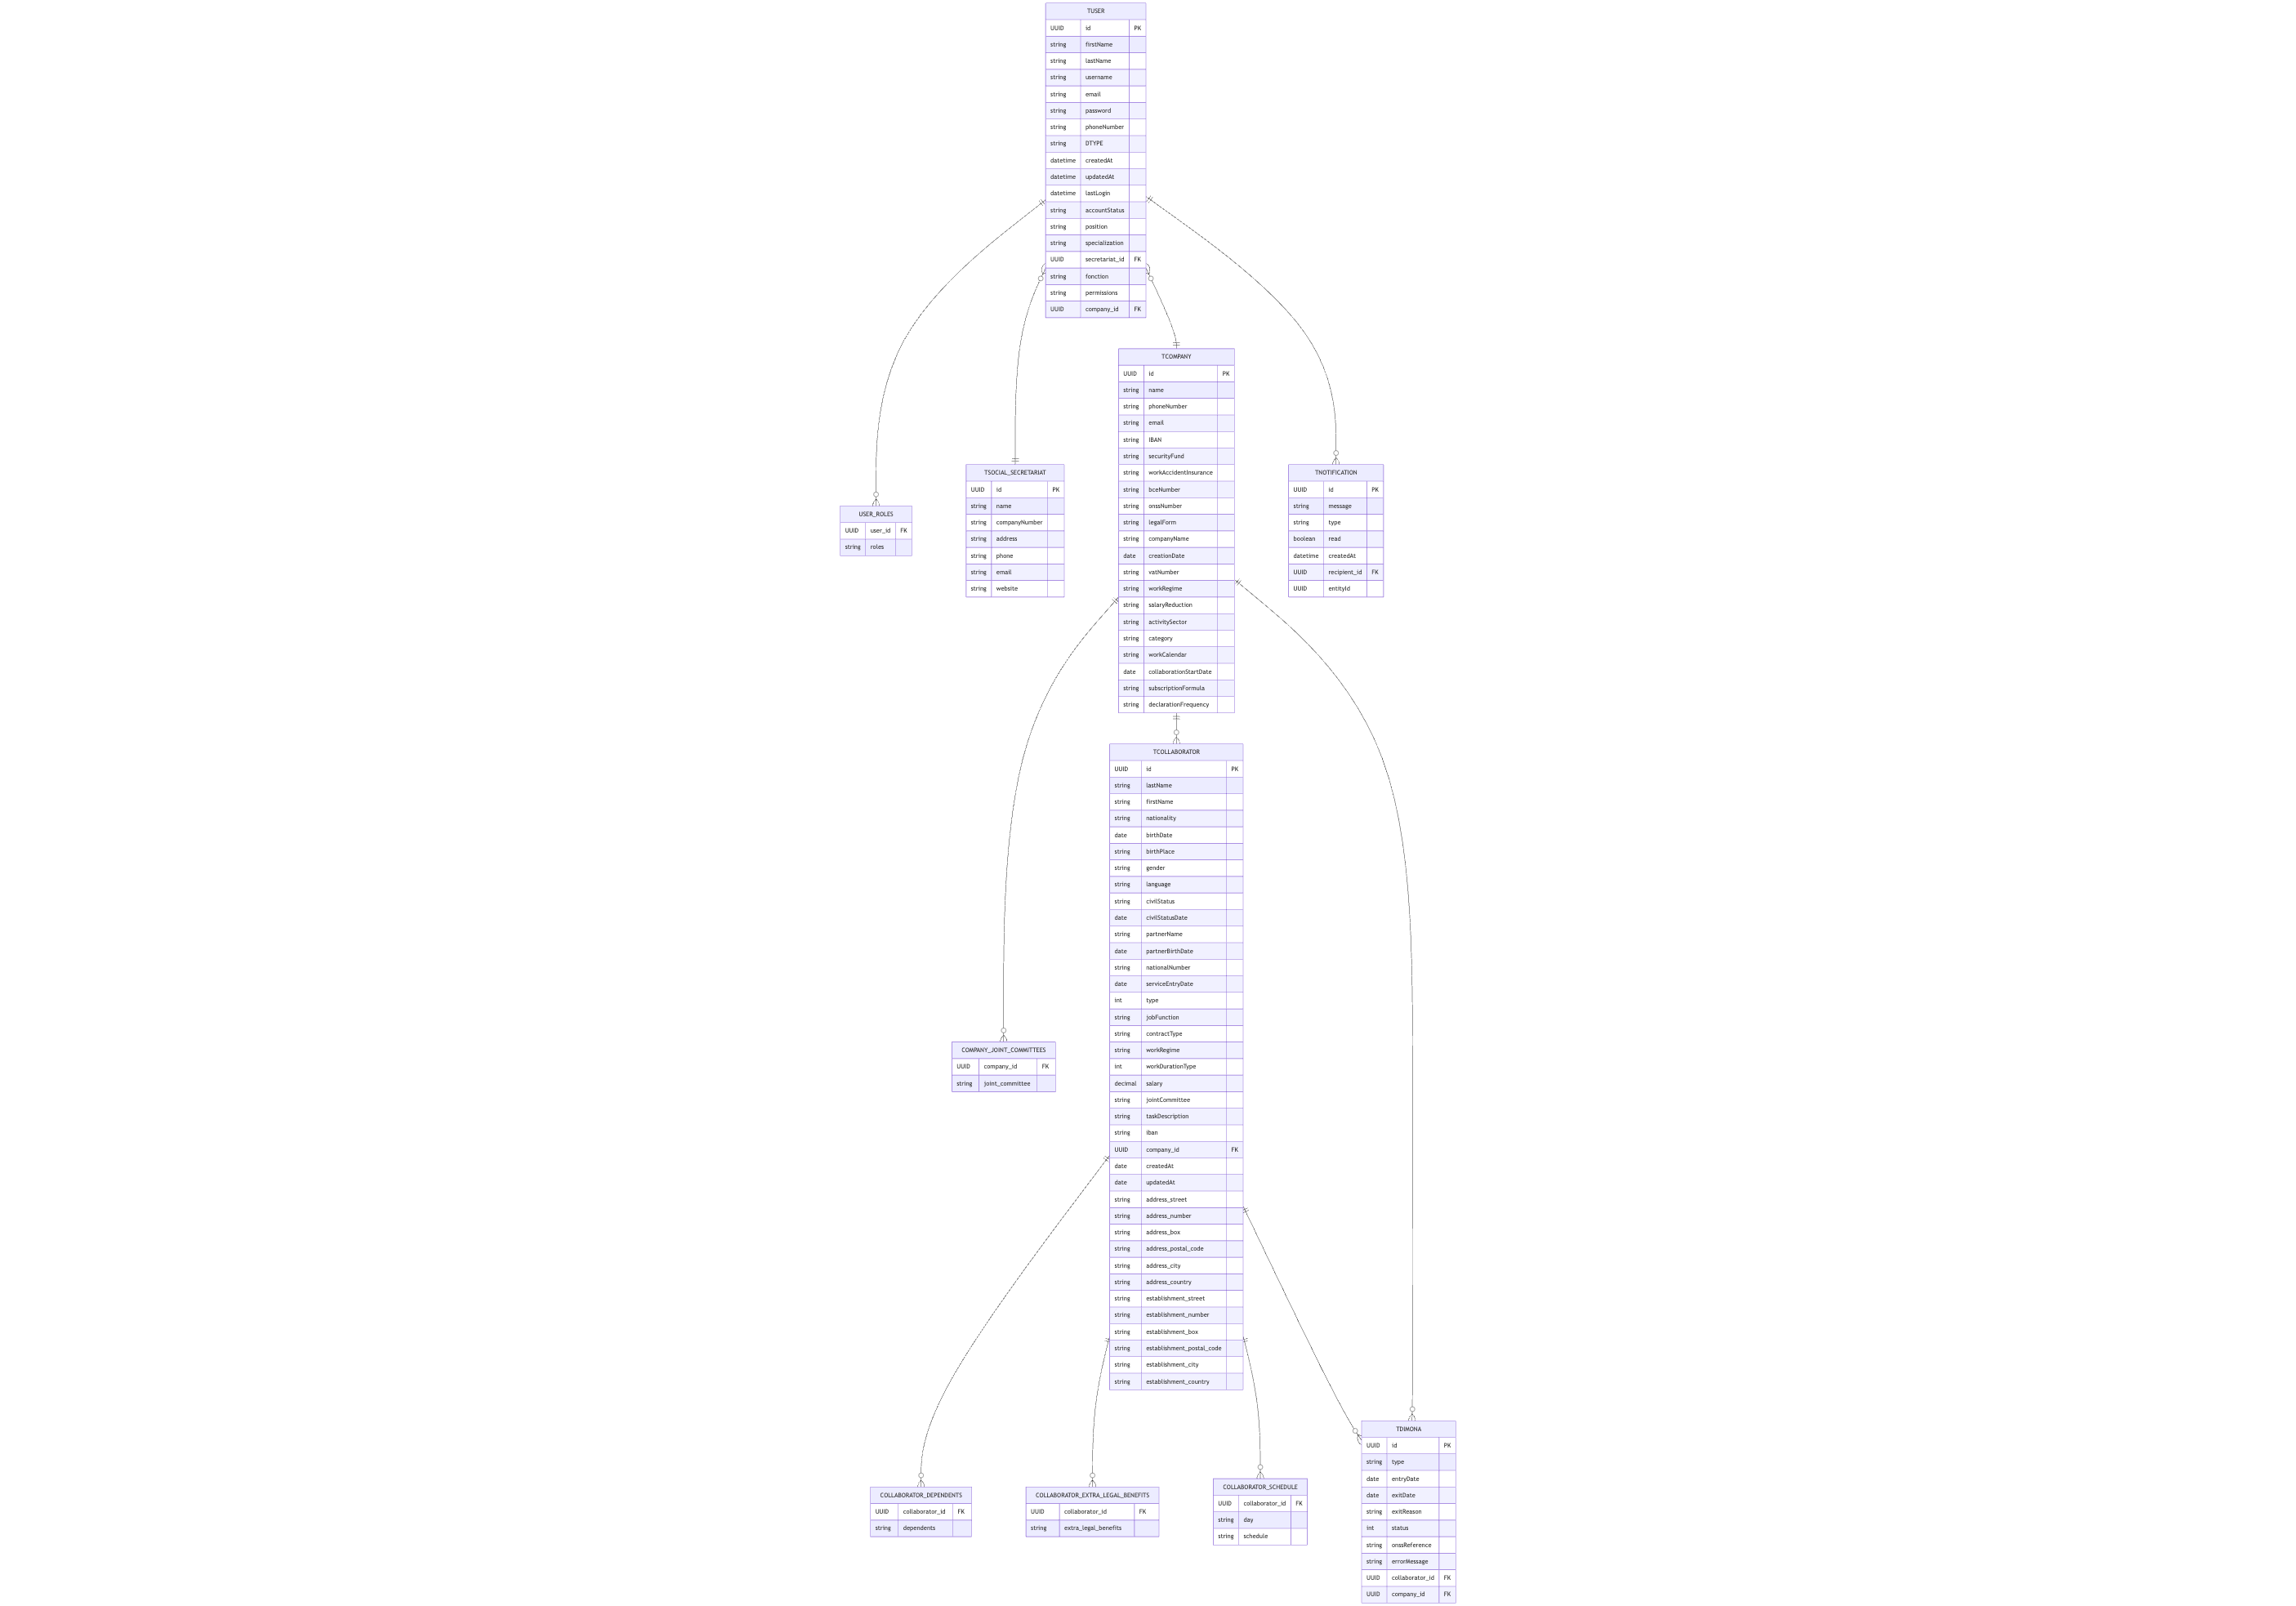
\includegraphics[width=0.9\textwidth]{ERD.png}
\caption{Diagramme d'entités relationnelles de SecuCom}
\end{figure}

\vspace{0.5cm}

\noindent Les principales entités de la base de données sont :

\begin{itemize}[leftmargin=*,label=\textcolor{darkgray}{$\bullet$},itemsep=0.3em]
  \item \textbf{TUSER} : Stocke les informations de base des utilisateurs (identifiant, email, mot de passe, nom, prénom, etc.). Cette table utilise l'héritage par une colonne discriminante (DTYPE) pour distinguer les différents types d'utilisateurs.

  \item \textbf{USER\_ROLES} : Table de jointure qui associe les utilisateurs à leurs rôles.

  \item \textbf{TSOCIAL\_SECRETARIAT} : Stocke les informations des secrétariats sociaux (nom, numéro d'entreprise, adresse, téléphone, email, site web).

  \item \textbf{TCOMPANY} : Stocke les informations des entreprises clientes (nom, téléphone, email, IBAN, numéro BCE, numéro ONSS, forme juridique, etc.).

  \item \textbf{COMPANY\_JOINT\_COMMITTEES} : Stocke les commissions paritaires associées aux entreprises.

  \item \textbf{TCOLLABORATOR} : Stocke les informations des travailleurs des entreprises clientes (nom, prénom, nationalité, date de naissance, lieu de naissance, genre, langue, état civil, numéro national, fonction, type de contrat, régime de travail, salaire, etc.).

  \item \textbf{COLLABORATOR\_DEPENDENTS} : Stocke les personnes à charge des collaborateurs.

  \item \textbf{COLLABORATOR\_EXTRA\_LEGAL\_BENEFITS} : Stocke les avantages extra-légaux des collaborateurs.

  \item \textbf{COLLABORATOR\_SCHEDULE} : Stocke les horaires de travail des collaborateurs.

  \item \textbf{TDIMONA} : Stocke les informations des déclarations DIMONA (type, date d'entrée, date de sortie, raison de sortie, statut, référence ONSS, message d'erreur, etc.).
  
  \item \textbf{TNOTIFICATION} : Stocke les notifications envoyées aux utilisateurs (message, type, statut de lecture, date de création, destinataire, référence à l'entité concernée).
\end{itemize}

\vspace{0.5cm}

\noindent Les relations entre ces entités sont les suivantes :

\begin{itemize}[leftmargin=*,label=\textcolor{darkgray}{$\bullet$},itemsep=0.3em]
  \item Un utilisateur peut avoir plusieurs rôles (relation one-to-many entre TUSER et USER\_ROLES).
  \item Un utilisateur peut être associé à un secrétariat social (relation many-to-one entre TUSER et TSOCIAL\_SECRETARIAT).
  \item Un utilisateur peut être associé à une entreprise (relation many-to-one entre TUSER et TCOMPANY).
  \item Une entreprise peut avoir plusieurs commissions paritaires (relation one-to-many entre TCOMPANY et COMPANY\_JOINT\_COMMITTEES).
  \item Une entreprise peut avoir plusieurs collaborateurs (relation one-to-many entre TCOMPANY et TCOLLABORATOR).
  \item Une entreprise peut avoir plusieurs déclarations DIMONA (relation one-to-many entre TCOMPANY et TDIMONA).
  \item Un collaborateur peut avoir plusieurs personnes à charge (relation one-to-many entre TCOLLABORATOR et COLLABORATOR\_DEPENDENTS).
  \item Un collaborateur peut avoir plusieurs avantages extra-légaux (relation one-to-many entre TCOLLABORATOR et COLLABORATOR\_EXTRA\_LEGAL\_BENEFITS).
  \item Un collaborateur peut avoir plusieurs horaires de travail (relation one-to-many entre TCOLLABORATOR et COLLABORATOR\_SCHEDULE).
  \item Un collaborateur peut avoir plusieurs déclarations DIMONA (relation one-to-many entre TCOLLABORATOR et TDIMONA).
  \item Un utilisateur peut recevoir plusieurs notifications (relation one-to-many entre TUSER et TNOTIFICATION).
\end{itemize}

\vspace{0.5cm}

\textbf{Champs obligatoires (NOT NULL):}
\begin{itemize}[leftmargin=*,label=\textcolor{darkgray}{$\bullet$},itemsep=0.3em]
  \item USER: firstName, lastName, username, email, password, roles, createdAt, accountStatus
  \item SOCIAL\_SECRETARIAT: name, companyNumber
  \item COMPANY: name
  \item COLLABORATOR: lastName, firstName, serviceEntryDate, company\_id, createdAt
  \item DIMONA: collaborator\_id, company\_id
\end{itemize}

\vspace{0.5cm}

\textbf{Contraintes d'unicité (UNIQUE):}
\begin{itemize}[leftmargin=*,label=\textcolor{darkgray}{$\bullet$},itemsep=0.3em]
  \item USER: username, email
  \item COMPANY: bceNumber, onssNumber, vatNumber
  \item COLLABORATOR: nationalNumber
\end{itemize}

\vspace{0.5cm}

\textbf{Types énumérés:}
\begin{itemize}[leftmargin=*,label=\textcolor{darkgray}{$\bullet$},itemsep=0.3em]
  \item USER.accountStatus: ACTIVE (défaut), INACTIVE, LOCKED, PENDING
  \item COLLABORATOR.type: EMPLOYEE, WORKER, FREELANCE, INTERN, STUDENT
  \item COLLABORATOR.workDurationType: FIXED, VARIABLE
  \item NOTIFICATION.type: DIMONA\_CREATED, DIMONA\_STATUS\_CHANGED, COLLABORATOR\_CREATED
\end{itemize}

\vspace{0.5cm}

\textbf{Suppression en cascade:}
\begin{itemize}[leftmargin=*,label=\textcolor{darkgray}{$\bullet$},itemsep=0.3em]
  \item La suppression d'une entreprise entraîne la suppression de tous ses contacts, collaborateurs et déclarations DIMONA associés.
  \item La suppression d'un collaborateur entraîne la suppression de toutes ses personnes à charge, avantages extra-légaux, horaires de travail et déclarations DIMONA associés.
  \item La suppression d'un utilisateur entraîne la suppression de toutes ses notifications associées.
\end{itemize}

\vspace{0.5cm}

\begin{tcolorbox}[
  title={\textbf{Modèle de données robuste}},
  colback=blue!5!white,
  colframe=primarycolor,
  fonttitle=\bfseries,
  boxrule=0.5mm,
  arc=2mm,
  left=6mm,
  right=6mm,
  top=6mm,
  bottom=6mm
]
Ce modèle de données permet de représenter efficacement les relations complexes entre les différentes entités du système, tout en assurant l'intégrité des données et la performance des requêtes. La structure relationnelle facilite la gestion des associations entre entreprises, collaborateurs et déclarations DIMONA, tout en maintenant une séparation claire des responsabilités. Les mécanismes de suppression en cascade garantissent la cohérence des données en évitant les références orphelines.
\end{tcolorbox}

\newpage

\section{Diagrammes de séquences}

\noindent Les diagrammes de séquence ci-dessous illustrent les interactions entre les différents composants du système \textbf{SecuCom} pour les cas d'utilisation clés. Ces diagrammes permettent de visualiser clairement les flux de communication entre les acteurs et le système.

\begin{note}
Les diagrammes de séquence sont particulièrement utiles pour comprendre la dynamique temporelle des interactions et identifier les points de communication critiques entre les différentes parties du système.
\end{note}

\subsection{Cas d'utilisation : Création d'une entreprise}

\noindent Le diagramme de séquence ci-dessous illustre le processus de création d'une entreprise dans le système \textbf{SecuCom}. Ce processus implique trois acteurs principaux : l'Administrateur, le Contact Entreprise et l'Employé du Secrétariat Social.

\begin{figure}[H]
\centering
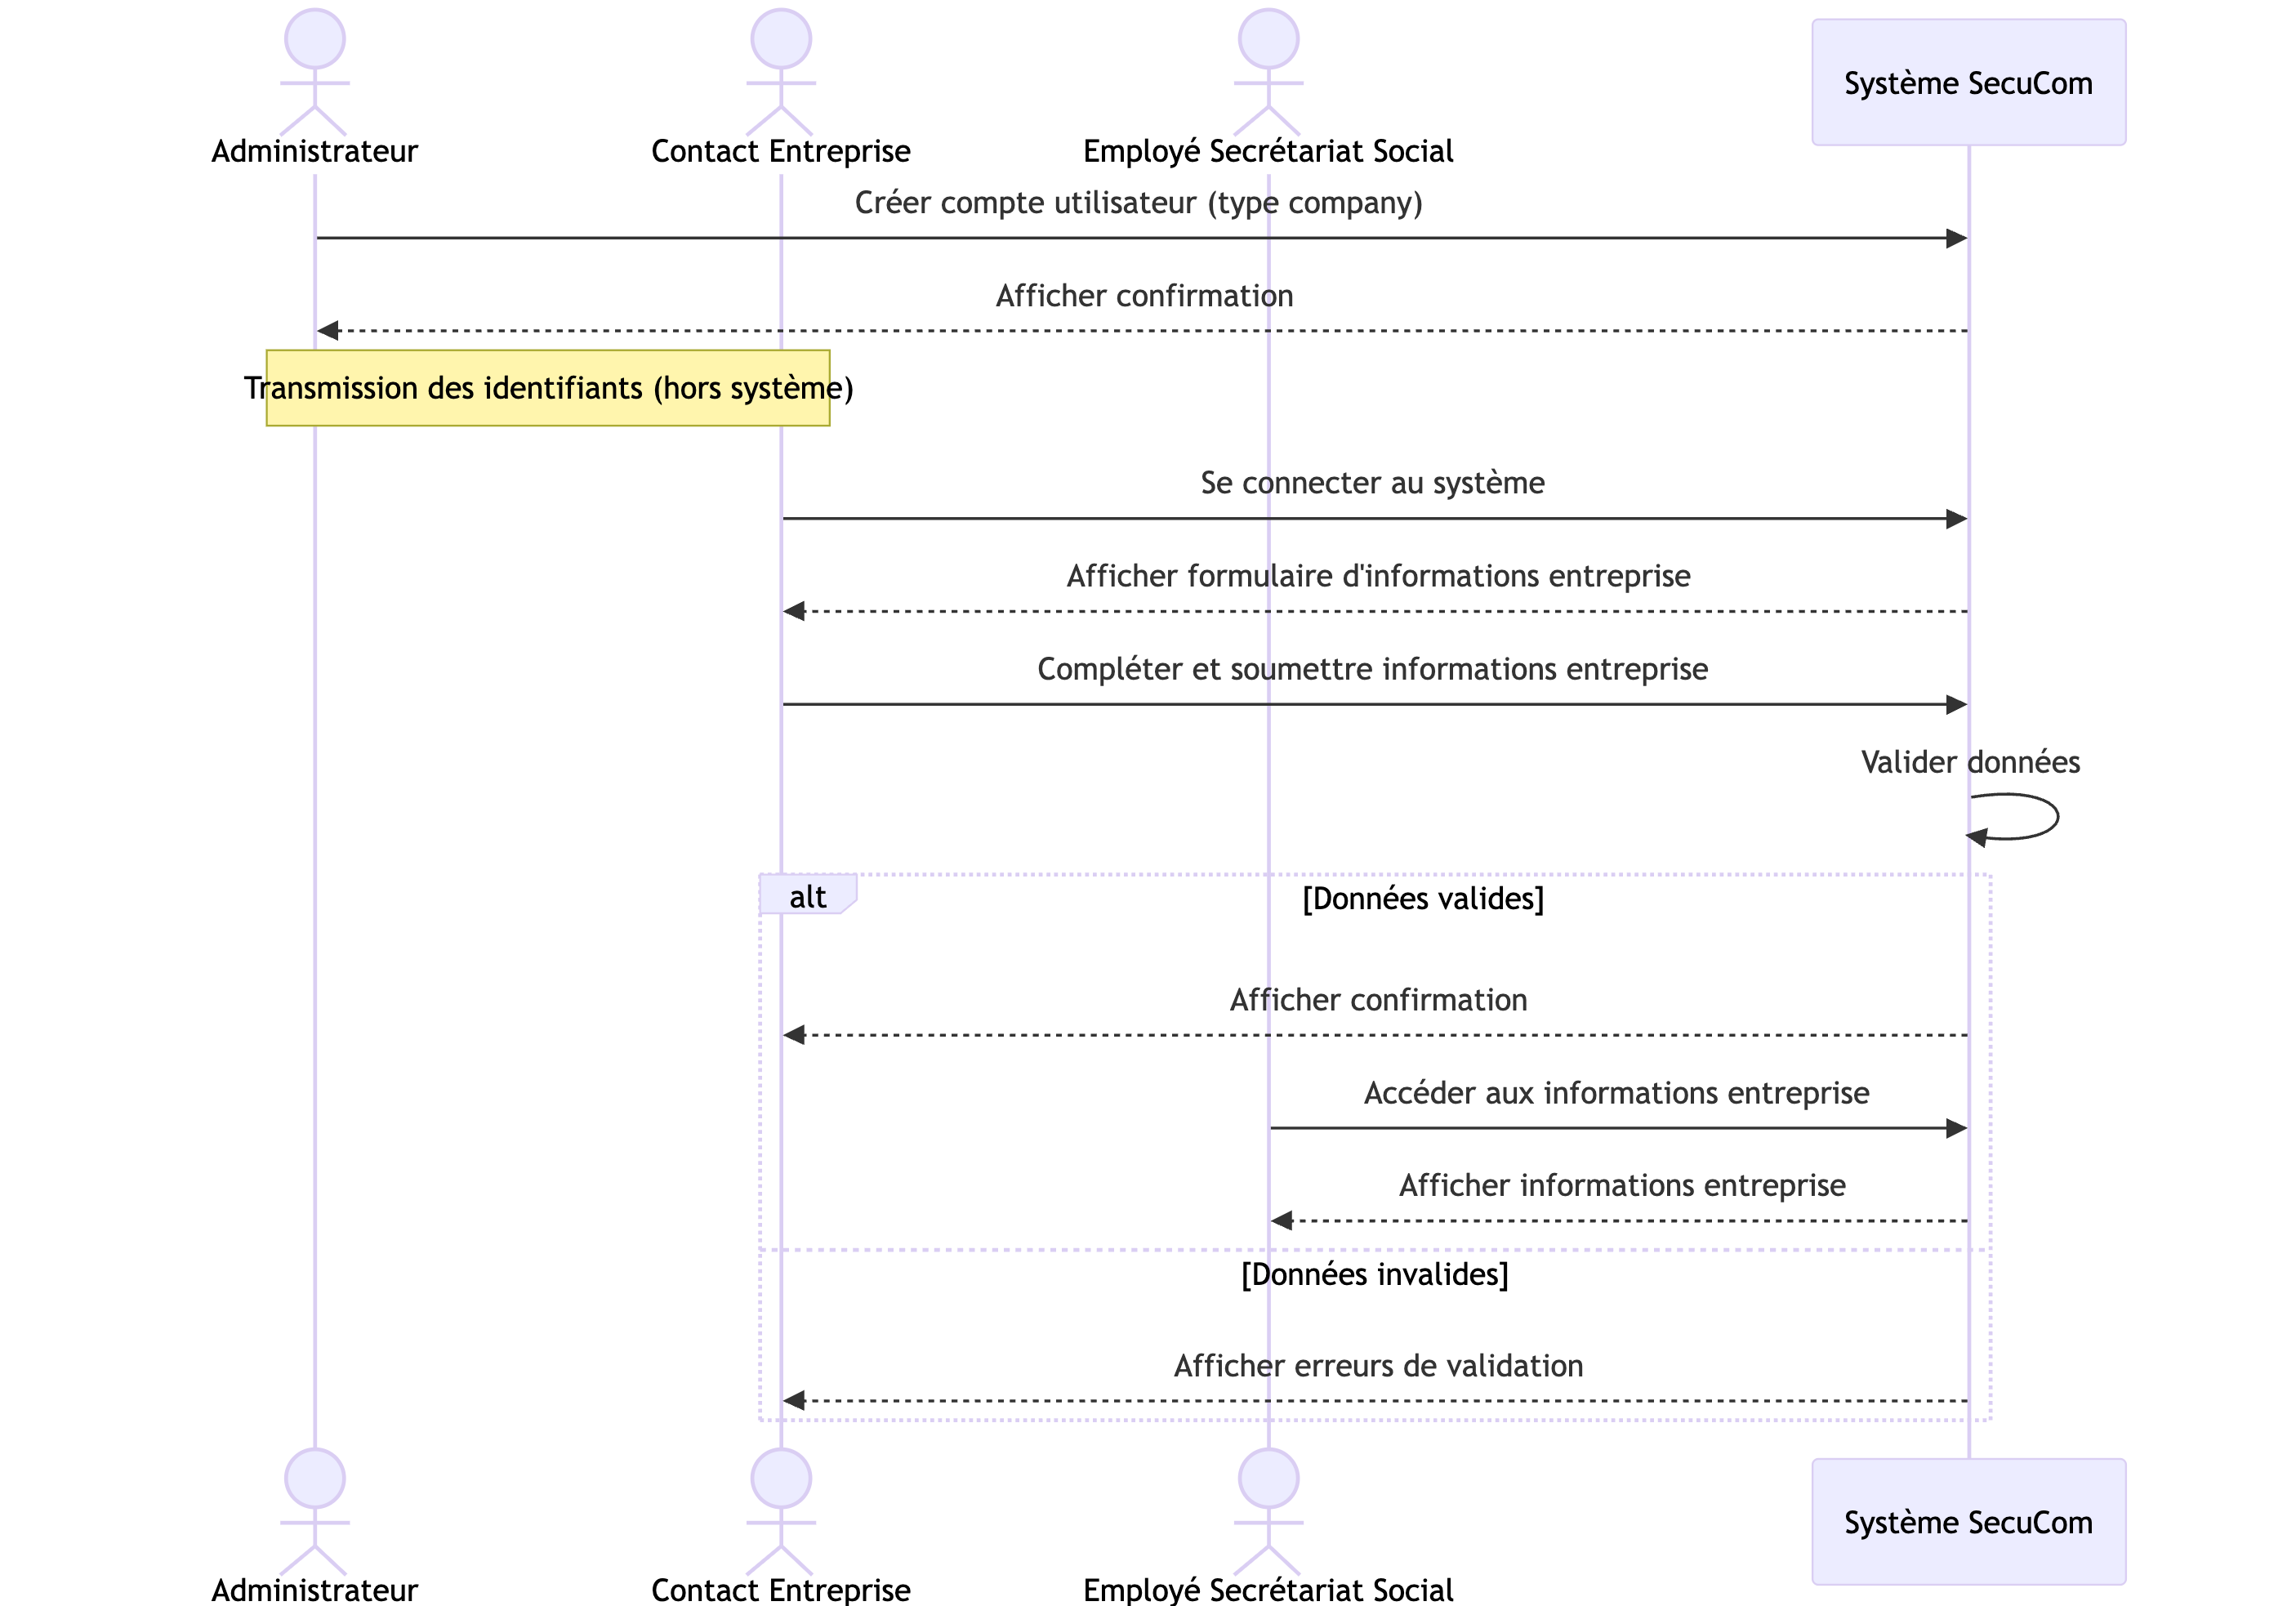
\includegraphics[width=0.9\textwidth]{SD_creation_entreprise.png}
\caption{Diagramme de séquence - Création d'une entreprise}
\end{figure}

\vspace{0.5cm}

\subsubsection{Description du processus}

\begin{enumerate}
  \item \textbf{Initialisation par l'Administrateur} :
    \begin{itemize}
      \item L'Administrateur crée un compte utilisateur de type "company" avec les données minimales obligatoires.
      \item Le système enregistre ces informations dans la base de données et confirme la création du compte.
    \end{itemize}

  \item \textbf{Transmission des identifiants} :
    \begin{itemize}
      \item L'Administrateur transmet les identifiants de connexion au Contact Entreprise (cette étape se déroule en dehors du système, par exemple par email ou téléphone).
    \end{itemize}

  \item \textbf{Complétion des informations par le Contact Entreprise} :
    \begin{itemize}
      \item Le Contact Entreprise se connecte au système avec les identifiants fournis.
      \item Le système affiche un formulaire permettant de compléter les informations de l'entreprise.
      \item Le Contact Entreprise saisit et soumet les informations complètes de son entreprise (nom, numéro BCE, numéro ONSS, numéro TVA, etc.).
      \item Le système valide les données soumises.
    \end{itemize}

  \item \textbf{Traitement des données} :
    \begin{itemize}
      \item Si les données sont valides, le système les enregistre dans la base de données et confirme l'enregistrement au Contact Entreprise.
      \item Si les données sont invalides, le système affiche les erreurs de validation au Contact Entreprise, qui doit les corriger et soumettre à nouveau.
    \end{itemize}

  \item \textbf{Accès par le Secrétariat Social} :
    \begin{itemize}
      \item L'Employé du Secrétariat Social peut accéder aux informations de l'entreprise.
      \item Le système récupère ces informations depuis la base de données et les affiche à l'Employé du Secrétariat Social.
    \end{itemize}
\end{enumerate}

\subsubsection{Avantages de cette approche}

Cette approche de création d'entreprise présente plusieurs avantages :
\begin{itemize}
  \item Elle responsabilise le Contact Entreprise pour la fourniture et la maintenance de ses propres informations.
  \item Elle réduit la charge administrative pour l'Administrateur et le Secrétariat Social.
  \item Elle améliore la précision des données puisqu'elles sont fournies directement par la source.
  \item Elle s'inscrit dans un modèle de self-service plus moderne et efficace.
  \item Elle facilite la scalabilité du système en permettant de gérer un plus grand nombre d'entreprises.
\end{itemize}

Ce processus constitue la première étape dans le cycle de vie d'une entreprise au sein du système SecuCom, et sert de fondation pour les autres cas d'utilisation comme l'ajout de collaborateurs et la création de déclarations DIMONA.

\subsection{Cas d'utilisation : Ajout d'un collaborateur}

\noindent Le diagramme de séquence ci-dessous illustre le processus d'ajout d'un collaborateur (employé) dans le système \textbf{SecuCom}. Ce processus implique plusieurs composants du système et inclut des validations importantes pour garantir l'intégrité des données.

\begin{figure}[H]
\centering
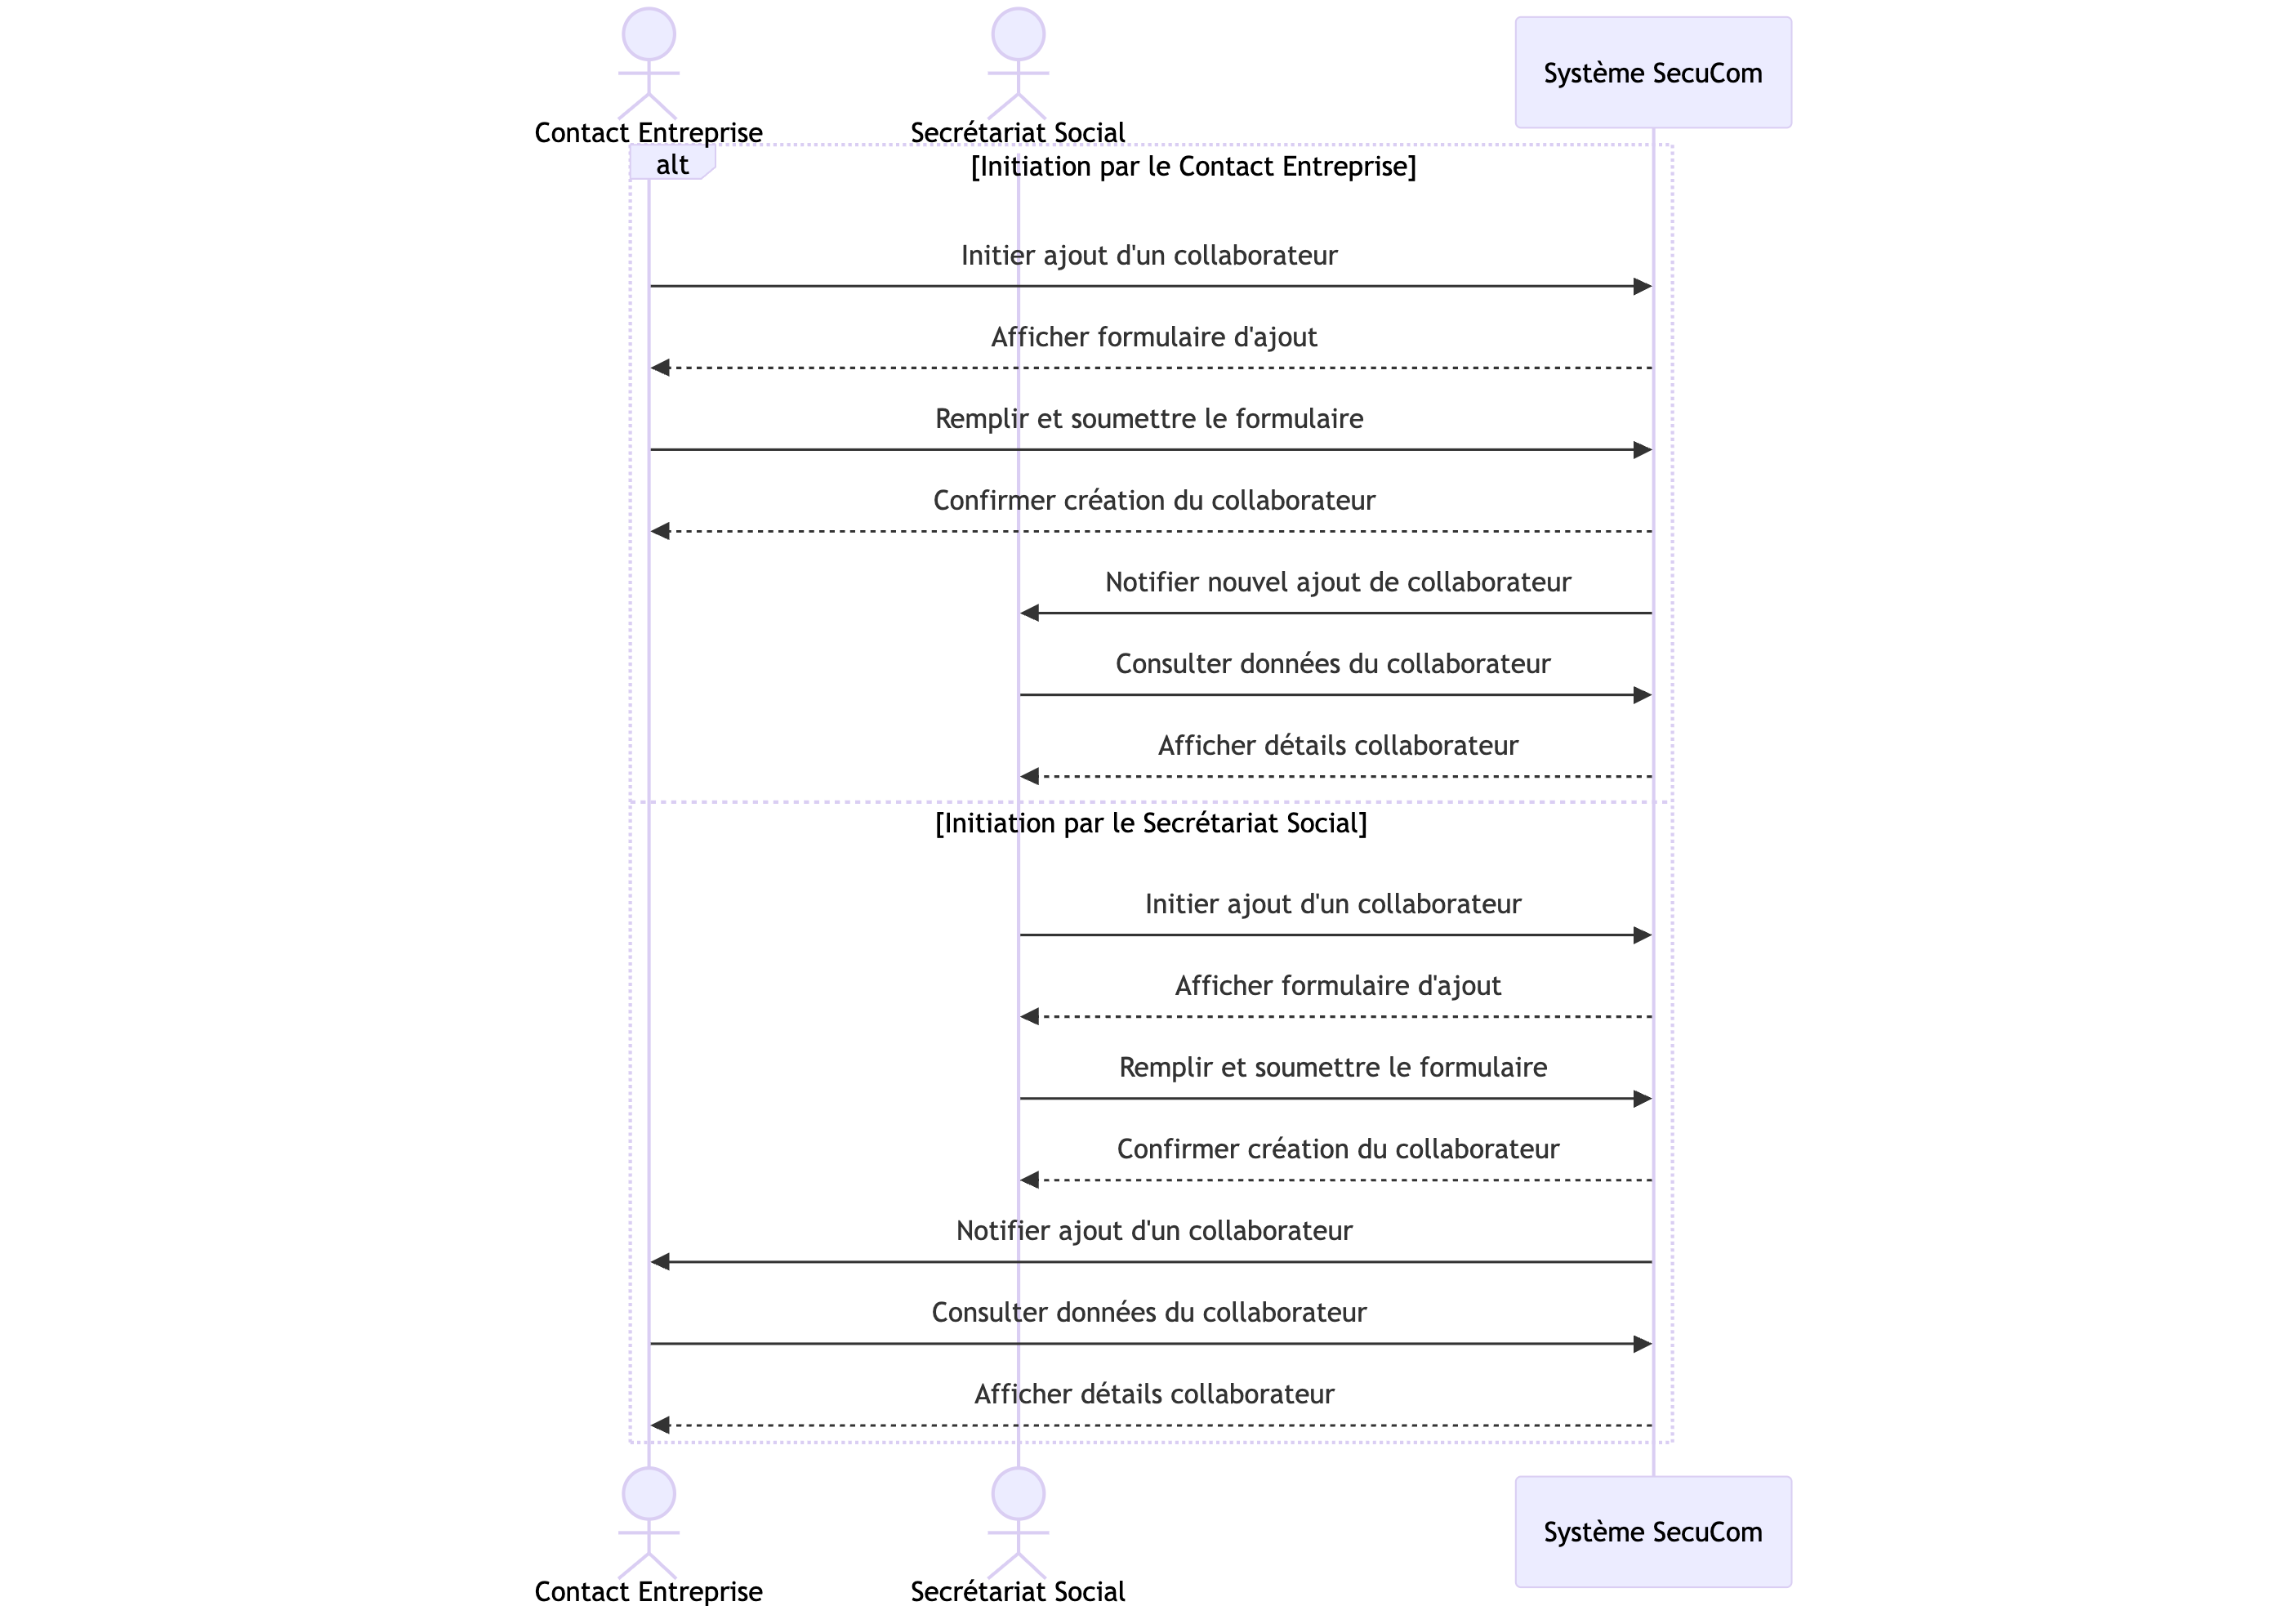
\includegraphics[width=0.9\textwidth]{SD_creation_collaborateur.png}
\caption{Diagramme de séquence - Ajout d'un collaborateur}
\end{figure}

\vspace{0.5cm}

\subsubsection{Description du processus}

\begin{enumerate}
  \item \textbf{Initiation de l'ajout} :
    \begin{itemize}
      \item \textbf{Scénario 1} : Le Contact Entreprise initie l'ajout d'un collaborateur, remplit le formulaire et soumet les données au système.
      \item \textbf{Scénario 2} : Le Secrétariat Social initie l'ajout d'un collaborateur, remplit le formulaire et soumet les données au système.
    \end{itemize}

  \item \textbf{Enregistrement des données} :
    \begin{itemize}
      \item Le système enregistre directement les informations du collaborateur dans la base de données.
      \item Une confirmation est envoyée à l'initiateur de la demande.
    \end{itemize}

  \item \textbf{Notification} :
    \begin{itemize}
      \item L'autre partie (celle qui n'a pas initié l'ajout) est notifiée de l'ajout du collaborateur.
      \item Elle peut consulter les détails du collaborateur ajouté.
    \end{itemize}
\end{enumerate}

\subsubsection{Aspects importants du processus}

Ce processus met en évidence plusieurs aspects importants du système SecuCom :

\begin{itemize}
  \item \textbf{Double flux d'initiation} : La flexibilité du système permet à deux types d'acteurs différents d'initier le processus selon les besoins et les préférences.
  \item \textbf{Simplicité du processus} : Le processus est simplifié pour permettre un ajout rapide et efficace des collaborateurs.
  \item \textbf{Communication bidirectionnelle} : Le système sert d'intermédiaire pour la communication entre le Contact Entreprise et le Secrétariat Social, facilitant le partage d'informations.
  \item \textbf{Traçabilité} : Toutes les étapes du processus sont enregistrées dans la base de données, permettant un suivi de l'historique des ajouts de collaborateurs.
\end{itemize}

L'ajout d'un collaborateur est une étape cruciale qui permet ensuite de procéder à d'autres opérations comme la création de déclarations DIMONA pour ce collaborateur.

\subsection{Cas d'utilisation : Création d'une déclaration DIMONA}

\noindent Le diagramme de séquence ci-dessous illustre le processus de création d'une déclaration DIMONA dans le système \textbf{SecuCom}. Ce processus peut être initié soit par le Contact Entreprise, soit par le Secrétariat Social, et implique une validation manuelle des données avant la soumission à l'ONSS.

\begin{figure}[H]
\centering
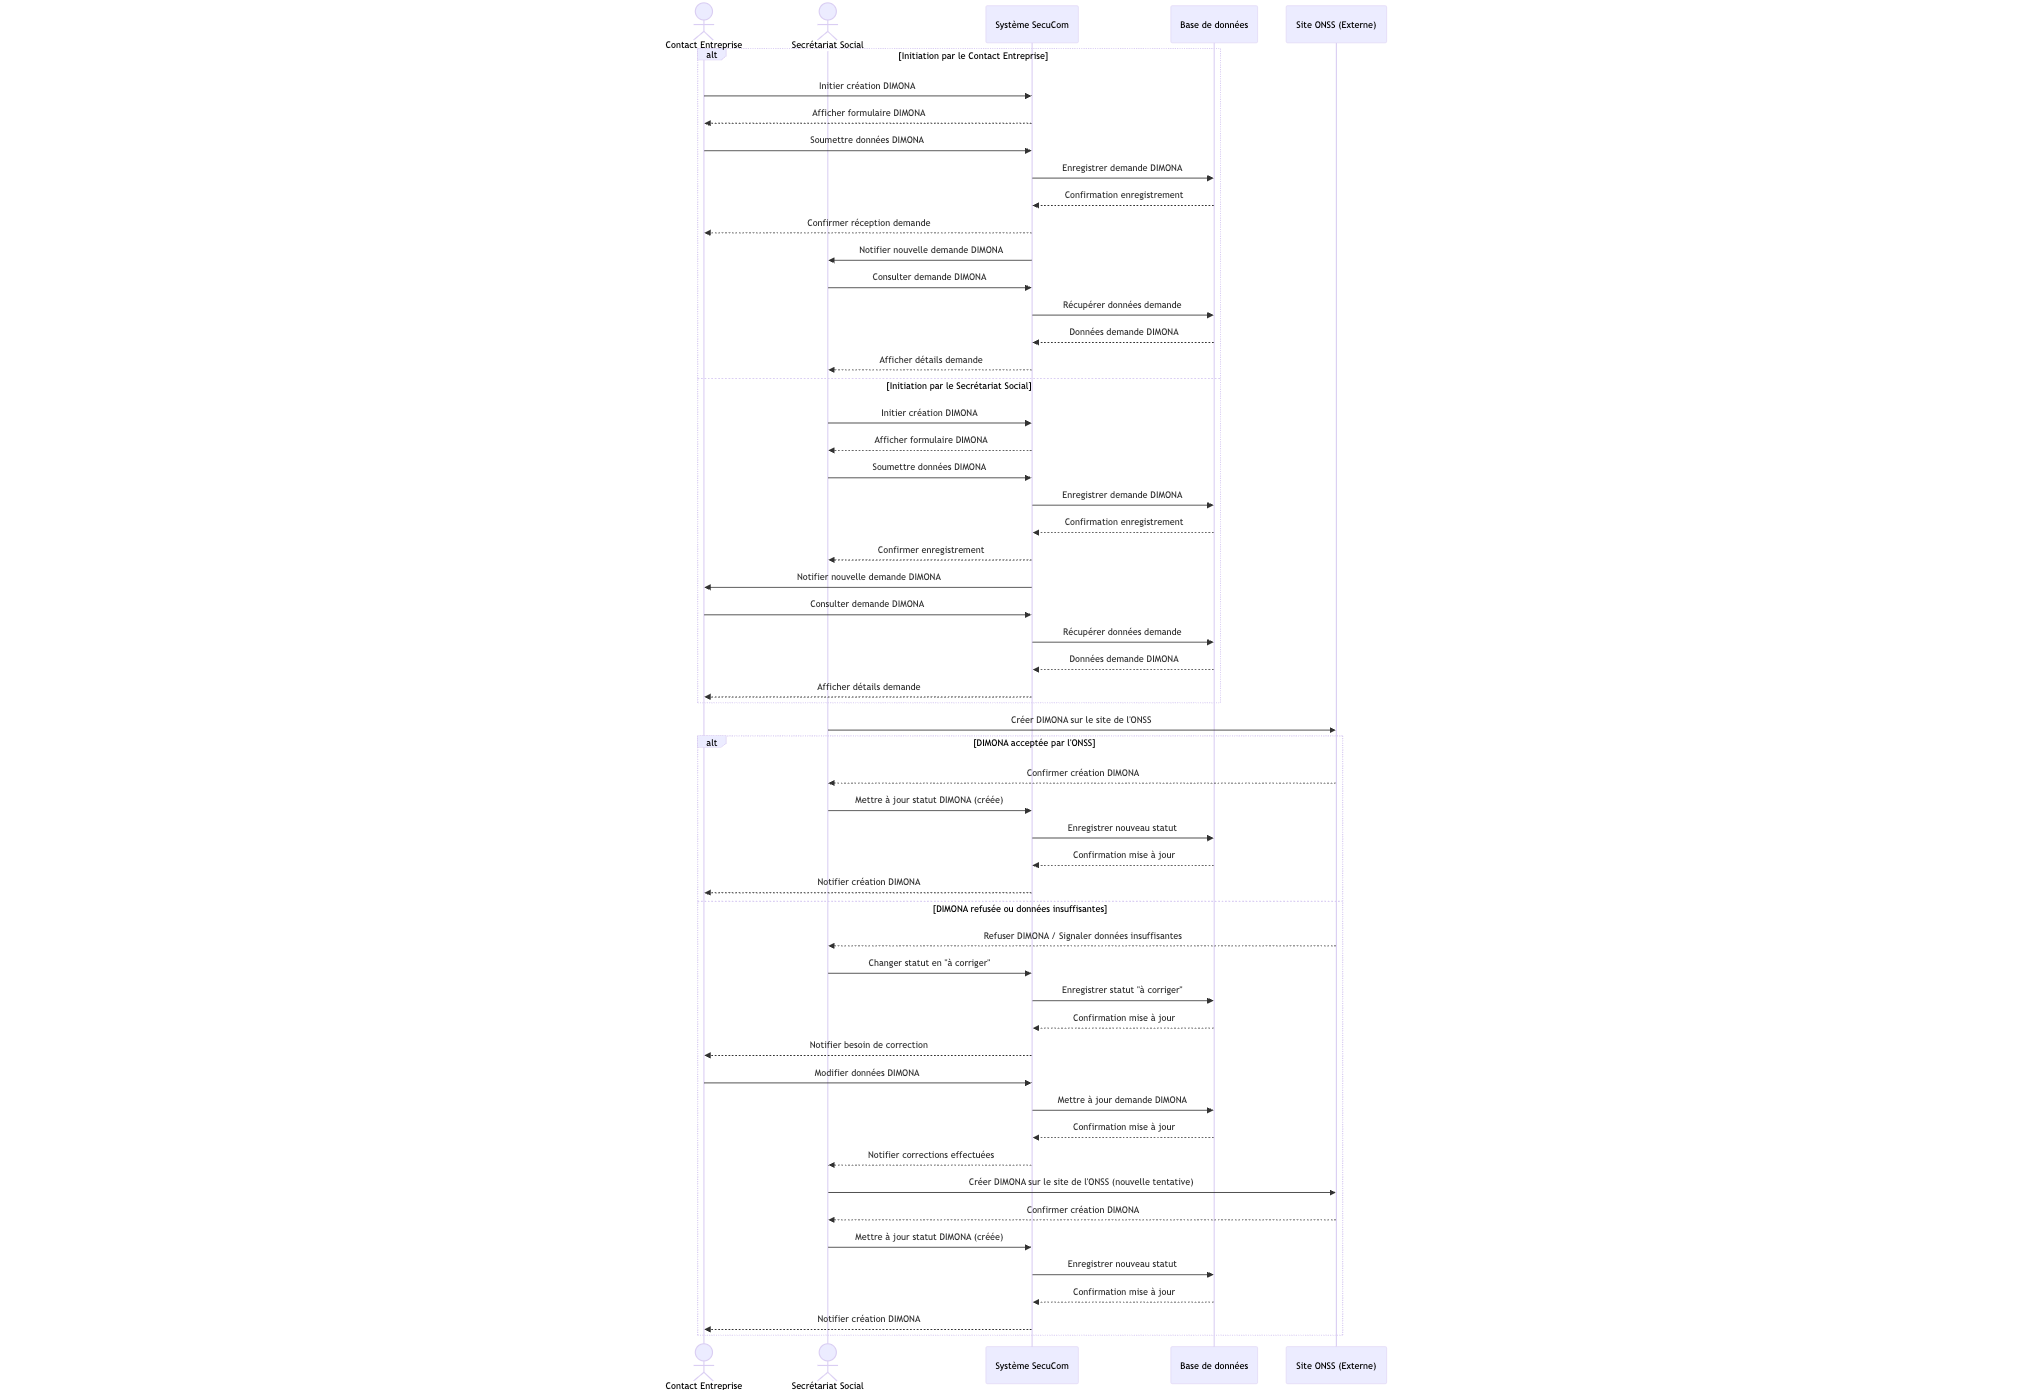
\includegraphics[width=0.9\textwidth]{SD_creation_dimona.png}
\caption{Diagramme de séquence - Création d'une déclaration DIMONA}
\end{figure}

\vspace{0.5cm}

\subsubsection{Description du processus}

\begin{enumerate}
  \item \textbf{Initiation de la demande} :
    \begin{itemize}
      \item \textbf{Scénario 1} : Le Contact Entreprise initie la création d'une déclaration DIMONA, remplit le formulaire et soumet les données au système.
      \item \textbf{Scénario 2} : Le Secrétariat Social initie la création d'une déclaration DIMONA, remplit le formulaire et soumet les données au système.
    \end{itemize}

  \item \textbf{Notification} :
    \begin{itemize}
      \item L'autre partie (celle qui n'a pas initié la demande) est notifiée de la nouvelle demande DIMONA.
      \item Elle peut consulter les détails de la demande.
    \end{itemize}

  \item \textbf{Création sur le site de l'ONSS} :
    \begin{itemize}
      \item Le Secrétariat Social crée la déclaration DIMONA sur le site officiel de l'ONSS.
    \end{itemize}

  \item \textbf{Traitement du résultat} :
    \begin{itemize}
      \item \textbf{Si la DIMONA est acceptée par l'ONSS} :
        \begin{itemize}
          \item L'ONSS confirme la création de la DIMONA.
          \item Le Secrétariat Social met à jour le statut dans le système.
          \item Le Contact Entreprise est notifié de la création effective de la DIMONA.
        \end{itemize}
      \item \textbf{Si la DIMONA est refusée ou les données sont insuffisantes} :
        \begin{itemize}
          \item L'ONSS refuse la DIMONA ou signale que les données sont insuffisantes.
          \item Le Secrétariat Social change le statut de la demande en "à corriger".
          \item Le Contact Entreprise est notifié et doit modifier les données.
          \item Après correction, le Secrétariat Social est notifié et fait une nouvelle tentative sur le site de l'ONSS.
          \item Une fois la DIMONA acceptée, le statut est mis à jour et le Contact Entreprise est notifié.
        \end{itemize}
    \end{itemize}
\end{enumerate}

\subsubsection{Aspects importants du processus}

\noindent Ce processus met en évidence plusieurs aspects importants du système \textbf{SecuCom} :

\begin{itemize}[leftmargin=*,label=\textcolor{darkgray}{$\bullet$},itemsep=0.3em]
  \item \textbf{Double flux d'initiation} : La flexibilité du système permet à deux types d'acteurs différents d'initier le processus selon les besoins et les préférences.
  \item \textbf{Gestion des refus et corrections} : Le système permet de gérer les cas où la DIMONA est refusée par l'ONSS, avec un mécanisme de notification et de correction.
  \item \textbf{Communication bidirectionnelle} : Le système sert d'intermédiaire pour la communication entre le Contact Entreprise et le Secrétariat Social.
  \item \textbf{Intégration avec les systèmes externes} : Le processus inclut l'interaction avec le site officiel de l'ONSS pour la création effective de la déclaration.
  \item \textbf{Traçabilité} : Le système maintient un suivi du statut des déclarations DIMONA, permettant aux parties concernées de connaître l'état actuel de chaque déclaration.
\end{itemize}

\vspace{0.5cm}

\begin{tcolorbox}[
  title={\textbf{Importance des déclarations DIMONA}},
  colback=blue!5!white,
  colframe=primarycolor,
  fonttitle=\bfseries,
  boxrule=0.5mm,
  arc=2mm,
  left=6mm,
  right=6mm,
  top=6mm,
  bottom=6mm
]
La création d'une déclaration DIMONA représente l'aboutissement du processus de gestion des collaborateurs, permettant de déclarer officiellement leur engagement auprès des autorités compétentes. Ce processus est crucial car il assure la conformité légale de l'entreprise et protège les droits des travailleurs en matière de sécurité sociale.
\end{tcolorbox}

% \section{Diagramme d'activité}

% Le diagramme d'activité ci-dessous illustre le flux de travail typique pour la gestion d'un collaborateur dans le système SecuCom, depuis sa création jusqu'à la génération de sa fiche de paie.

% Ce flux de travail comprend plusieurs étapes :
% \begin{enumerate}
%   \item Création de l'entreprise cliente
%   \item Ajout d'un contact pour l'entreprise
%   \item Ajout d'un collaborateur à l'entreprise
%   \item Création d'une déclaration DIMONA pour le collaborateur
%   \item Suivi du statut de la déclaration DIMONA, qui peut être :
%      \begin{itemize}
%        \item En attente
%        \item Acceptée
%        \item Rejetée (nécessitant une correction et une nouvelle soumission)
%      \end{itemize}
%   \item Enregistrement des prestations du collaborateur
%   \item Génération de la fiche de paie
%   \item Archivage et envoi des documents
% \end{enumerate}

% Chaque étape du flux peut être réalisée par différents acteurs (employé du secrétariat, contact d'entreprise) selon leurs permissions dans le système. Le flux n'est pas strictement linéaire et peut comporter des boucles ou des branches conditionnelles selon les besoins spécifiques de chaque cas.

% Ce diagramme d'activité permet de visualiser clairement le processus métier global et d'identifier les points d'interaction entre les différents acteurs et le système.
